%%%%%%%%%%%%%%%%%%%%%%%%%%%%%%%%%%%%%%%%%
% St Sectioned Assignment
% LaTeX Template
% Version 1.0 (5/5/12)
%
% This template has been downloaded from:
% http://www.LaTeXTemplates.com
%
% Original author:
% Frits Wenneker (http://www.howtotex.com)
%
% License:
% CC BY-NC-SA 3.0 (http://creativecommons.org/licenses/by-nc-sa/3.0/)
%
%%%%%%%%%%%%%%%%%%%%%%%%%%%%%%%%%%%%%%%%%

%----------------------------------------------------------------------------------------
%	PACKAGES AND OTHER DOCUMENT CONFIGURATIONS
%----------------------------------------------------------------------------------------

\documentclass[paper=a4, fontsize=11pt]{scrartcl} % A4 paper and 11pt font size

\usepackage[T1]{fontenc} % Use 8-bit encoding that has 256 glyphs
%\usepackage{fourier} % Use the Adobe Utopia font for the document - comment this line to return to the LaTeX default
\usepackage[english]{babel} % English language/hyphenation
\usepackage{amsmath,amsfonts,amsthm} % Math packages

\usepackage{lipsum} % Used for inserting dummy 'Lorem ipsum' text into the template
\usepackage{graphicx}

\usepackage{sectsty} % Allows customizing section commands
\allsectionsfont{\centering \normalfont\scshape} % Make all sections centered, the default font and small caps

\usepackage{hyperref}


\usepackage{fancyhdr} % Custom headers and footers
\pagestyle{fancyplain} % Makes all pages in the document conform to the custom headers and footers
\renewcommand{\headrulewidth}{0pt} % Remove header underlines
\renewcommand{\footrulewidth}{0pt} % Remove footer underlines
\setlength{\headheight}{13.6pt} % Customize the height of the header

\numberwithin{equation}{section} % Number equations within sections (i.e. 1.1, 1.2, 2.1, 2.2 instead of 1, 2, 3, 4)
\numberwithin{figure}{section} % Number figures within sections (i.e. 1.1, 1.2, 2.1, 2.2 instead of 1, 2, 3, 4)
\numberwithin{table}{section} % Number tables within sections (i.e. 1.1, 1.2, 2.1, 2.2 instead of 1, 2, 3, 4)

\setlength\parindent{0pt} % Removes all indentation from paragraphs - comment this line for an assignment with lots of text

%----------------------------------------------------------------------------------------
%	TITLE SECTION
%----------------------------------------------------------------------------------------

\newcommand{\horrule}[1]{\rule{\linewidth}{#1}} % Create horizontal rule command with 1 argument of height



\renewcommand{\vec}[1]{\textbf{#1}}
\newcommand{\ssvec}[1]{\textsf{\textbf{#1}}}

\newcommand{\veca}{\vec{a}}
\newcommand{\vecx}{\vec{x}}
\newcommand{\vecy}{\vec{y}}
\newcommand{\vecz}{\vec{z}}

\newcommand{\rveca}{\ssvec{a}}
\newcommand{\rvecx}{\ssvec{x}}
\newcommand{\rvecy}{\ssvec{y}}
\newcommand{\rvecz}{\ssvec{z}}

\newcommand{\yone}{\textsf{y}_1}
\newcommand{\ytwo}{\textsf{y}_2}

\newcommand*{\everymodeprime}{\ensuremath{\prime}}

\begin{document}


%----------------------------------------------------------------------------------------
%	PROBLEM 1
%----------------------------------------------------------------------------------------
\newpage

NOTE: the goal is to be headed in right direction for research, and also have some subset/version be implementable before June 15 (Nick's Roy's deadline) \\

\textbf{Introduction}
\\

With the high-speed autonomous flight problem, the need is for controllers that are ``reactive'' in that they respond almost instantaneously without a deliberative, slow planning process, but consider robustness in a principled way and are not suspect to chattering.\\

This formulation explores the use of a library of control actions from which actions are stubbornly chosen.   By not building a map over time, and by avoiding ``trajectory-tracking'' in the sense of controlling along a nominal, planned trajectory, this approach is minimally dependent on state estimation: position estimates are not needed, and velocity estimates are expected to be considerably uncertain.  Rather than building a map, we always consider the instantaneous depth image in the vehicle's relative coordinates.  The benefits of stubborn control from a library include:
\begin{itemize}
\item The ``stubbornness'' of the control can be an option for encoding hysteresis, rather than building a map.
\item A discrete library has practical benefits for avoiding optimization of the non-covex ``should I turn left or right?'' problem.
\item With a finite library, the online decision is as simple as evaluating the finite options.
\end{itemize}

As a comparison for the stubborn control idea, an alternative approach using a small local map is also considered.  With this local map option, the instantaneous depth image is augmented with previous $N$ depth measurements whose positions and covariances are propagated via the vehicle's motion (for which a position + orientation estimate is desired).\\

Central to both of these approaches is the trade-off between minimizing the chance of collision, while also making progress towards the goal.  Accordingly, the simple summary of the stubborn formulation is that the online control choice is the action, $\mathbb{A}_i$, that minimizes the sum of costs (where each $k$ is just a weighting factor):

$$ \underset{i}{\text{argmin}} \bigg[ k_{tg}\big[ cost(\mathbb{A}_i)_{\text{towards goal}}  \big]+  k_{s} \big[ cost(\mathbb{A}_i)_{\text{switching}} \big]+   k_{pc}\big[ cost(\mathbb{A}_i)_{\text{probabilistic collision}} \big]  \bigg]$$

The word action rather than trajectory has been used because the actions are chosen from a discrete sampling of the input space, which for the model we describe is just of dimension 3, rather than the full state space, which for our model is of dimension 12.  We assume here only that the $cost_{\text{towards goal}}$ function is provided by some higher-level system, which could for example use the global position estimate to navigate us towards a global goal.\\




This is meant as a first complete description and there are many opportunities for improving and increasing complexity, including model complexity and including a Bayesian update for control decisions as another way to include hysteresis.\\  

%\horrule{1pt} 
%\\


\textbf{Assumptions of problem}
\\

Our actual hardware system is a quadrotor UAV with all onboard sensing and computation, and most relevant parameters of this system are: 
\begin{itemize}
\item Up to 15 m/s velocity towards obstacles
\item At full speed, expected stopping distance is in the range of 20+ m
\item A 5 m range, 120 x 160 depth image is available at 30 Hz
\item Estimates for x, y, z linear velocities and covariances are available at 30 Hz
\item Due to the difficulty of state estimation at high speeds, the uncertainty for the velocity estimates are expected to be high: perhaps as high as +/- 5 m/s for 1-$\sigma$.  (Note that even though a graph-based state estimation is used (iSAM), internally the state estimator linearizes the graph to use a Gauss-Newton solver, and so Gaussian covariances are straightforward to provide.)
\item A higher level system provides the ``global navigation function'' which evaluates $cost(\mathbb{A}_i)_{\text{towards goal}} $ for us.
\item An inner-loop attitude controller will stabilize desired attitude and thrust setpoints at 200+ Hz with the IMU alone for attitude estimation. (This is very practical, due to high IMU rates and sufficiency for estimating attitudes.)
\end{itemize}

Note that at maximum speed, the stopping distance is larger than the range of the depth sensing information.  Hence the primary goal is, to the best of the quadrotor's noisy information, swerve to avoid obstacles. \textit{At full speed, stopping for safety is not an option. Swerving towards the most dynamically feasible open area is the only option}.  At speeds low enough such that the stopping distance is less than the sensing horizon, however, we also want a system that will naturally choose stopping. \\

An assumption we make at least in this initial approach is that the quadrotor plant in feedback with the inner-loop attitude controller can be approximated by a simple double integrator model with drag.  Although this does not capture the attitude dynamics of the vehicle (it takes time for the vehicle to switch from a roll-right to a roll-left), the attitude dynamics of the vehicle are much faster than the velocity dynamics.  There are advantages for us starting with this simple linear model that has independence of $x, y, and z$ (both for computational complexity, and for reasoning about), and it is my guess that this simple model can be taken far before its limits are shown. It is, however, an approximation that is inherent to the simplicity of a quadrotor.

\begin{figure}
  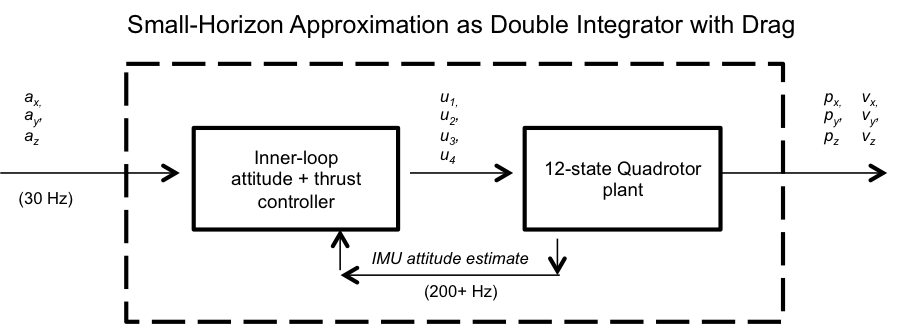
\includegraphics[width=\linewidth]{double_integrator_approximation.png}
  \caption{Dynamics approximation considered: the quadrotor is modeled in feedback with the inner loop attitude and thrust controller.}
  \label{fig:boat1}
\end{figure}

\textbf{Approach}
\\

Inputs required are: (i) an instantaneous depth image containing $r \times c = M$ points in relative coordinates $x_i, y_i, z_i$ and each with covariance $\Sigma_{d.r.}$, (ii) estimates for the linear $x, y, z$ velocities with covariance $\Sigma_{v_0}$, and (iii) the $x,y,z$ location of a local goal.  As a first, simple approach, the $cost(\mathbb{A}_i)_{\text{towards goal}} $ can be approximated via Euclidean distance to the local goal.\\

The actions considered live in the input space to the double integrator approximation: accelerations in $\mathbb{R}^3$.  To create the bins for $a_x$ and $a_y$ each, we approximate the maximum horizontal acceleration and sample over possible horizontal accelerations around a circle in the horizontal plane.   The max horizontal acceleration is approximated as the maximum thrust vector ($T_{max}$, easy to measure) angled just enough to compensate for gravity: $a_{max} = \frac{ \sqrt{ T_{max}^2 + (mg)^2}}{m}$.  By sampling both over the horizontal acceleration with just a few discretizations (for example, [$a_{max}, 0.6a_{max}, 0.3*a_{max} ]$) and just 8 evenly spaced $\theta$ over $[0, 2\pi]$, this yields a useful 24 options in the horizontal plane.  The figure below is a depiction of forming the horizontal $[a_x, a_y]$ bins.  For the bins where the maximum horizontal acceleration is used, we only use $a_z = 0$ since thrust is already saturated, but when thrust is not saturated we add up vertical options as well $a_z = [-a_{vert}, 0, a_{vert}]$. This makes for a total of 56 $[a_x, a_y, a_z]$ actions for the quadrotor to consider.\\

\begin{figure}
  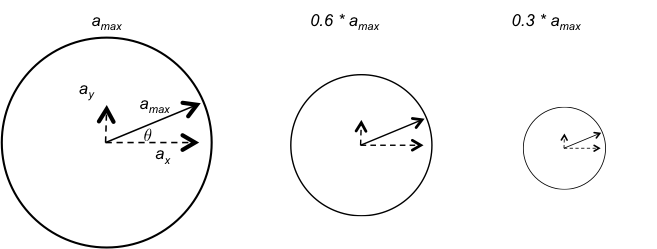
\includegraphics[width=\linewidth]{horizontal_actions.png}
  \caption{Formation of horizontal actions from sampling over thrust-scaled circles in the horizontal plane.}
  \label{fig:boat1}
\end{figure}

Over the small receding planning horizon (we use a finite time horizon $t_f = 500$ ms at least to start out), paths through configuration space can be trivially calculated at any moment, due to the simple constant-acceleration point-mass model (double integrator).  A benefit of this simple model is that due to the constant accelerations and the independence of $x, y, z$, we do not even need to sequentially forward-simulate a trajectory with the state, instead we can calculate directly the position $\mathbf{p}(t)$ of the robot for any time.  Calculating each position of each action at each time is 100\% parallelizable.

$$ \textbf{p}_i(t) = \frac{1}{2} \textbf{a}_i t^2 + \mathbf{v}_0 t \ \ \ \text{for action} \  \mathbb{A}_i$$

Note that initial positions are always considered to be $[0,0,0]$, since we are in the robot's relative coordinates.  The linear velocity estimates $\mathbf{v}_0$ coming from our state estimation system are the random variables, as will be discussed in the probabilistic collision calculations.\\

The on-line decision requires the evaluation of each of the possible actions:
$$ cost(\mathbb{A}_i)_{\text{total}} = k_{tg}\big[ cost(\mathbb{A}_i)_{\text{towards goal}}  \big]+  k_{s} \big[ cost(\mathbb{A}_i)_{\text{switching}} \big]+   k_{pc}\big[ cost(\mathbb{A}_i)_{\text{probabilistic collision}} \big] $$

The first and second terms, the costs towards the goal and the switching (stubborn) costs are trivial to evaluate.  As a first approximation we can evaluate the cost towards the goal as the Euclidean distance to the provided local goal:

$$cost(\mathbb{A}_i)_{\text{towards goal}} = || \mathbf{p}_i(t_f) - \mathbf{p}_{goal} ||_2 $$

And the cost of switching can be defined as a norm in the input space (desired accelerations) between the previous input and the considered new input.  We guess the 1-norm is reasonable:

$$cost(\mathbb{A}_i)_{\text{switching}} = || \textbf{a}_i - \textbf{a}_{previous} ||_1 $$

The final term is overwhelmingly the most computationally complex.  It is actually trivial, due to products of Gaussians also being Gaussians, to calculate the probability density for any (i) single action, (ii) single point in time, with (iii) a single point in the point cloud.  With the simple point-mass model, every single one of these computations is parallelizable.\\

For each $\mathbb{A}_i$ at each $t$, we assume that the robot's future position is a Gaussian distribution: 

$$\mathbf{p}(t) \sim N(\mathbf{\hat{p}}(t), \Sigma_p(t))$$

Where the covariance of the position is due to the appropriate scaling of the initial velocity covariance (recall $ \textbf{p}_i(t) = \frac{1}{2} \textbf{a}_i t^2 + \mathbf{v}_0 t$):

$$ \Sigma_{p_i(t)} = t^2 \Sigma_{v_0}$$

We also have a Gaussian distribution on each of the points from each of the $j$ depth returns, $\mathbf{p}_{j} \sim N(\mathbf{\hat{p}}_{j}, \Sigma_{d.r.})$.  The $\Sigma_{d.r.}$ can be approximated as uniform for each point in the point cloud, and estimated from sensor data or a sensor specification sheet.\\

It is known that the product of two Gaussian distributions is itself a Gaussian, and independence of the robot position distribution and the sensor distribution is a fair assumption, so we have for the joint distribution:

$$ p(\text{collision}_{i,j,t}) = \frac{1}{\sqrt{\text{det}}(2 \pi \Sigma_{C(i, t)})} \exp \big[  -\frac{1}{2}(\mathbf{\hat{p}}(t) - \mathbf{\hat{p}}_{j})^T \Sigma_{C(i, t)}^{-1} (\mathbf{\hat{p}}(t) - \mathbf{\hat{p}}_{j}) \big] $$

Where $\Sigma_{C(i, t)} = \Sigma_{p_i(t)} + \Sigma_{d.r.}$.  The above only gives the probability density for a given point (which is measure 0), rather than a integral of the density over some volume.  We note that in chance-constrained programming (Toit 2012), because calculating an actual probability is desired in order to pose a chance constraint, they approximate the integral with a small-sphere approximation, multiplying the volume of the robot $V_r$ by the probability density at the mean.  For us, however, since the probabilistic aspect is considered as part of the objective, the volume would just be a linear scaling for each and every probability calculated, and so it is not needed.\\

For a given (i) single action, (ii) single point in time, and (iii) a single point in the point cloud, the above (with a small volume approximation) could actually be considered a probability (between [0,1]).  Since we want to calculate a cost of collision for (i) a single action, but over all future time and over all possible points in the point cloud, we want a metric which includes all time and all points.  Although it is not a ``probability'' (not between [0,1]), we sum all of the individual probabilities for a given action:

$$cost(\mathbb{A}_i)_{\text{probabilistic collision}} = \sum_j \sum_t p(\text{collision}_{i,j,t}) $$

Which can be thought of as an un-normalized (linear scaling doesn't matter) weighted average of the probability of collision.

We now consider the complexity of this naive algorithm.  Clearly, the complexity grows naively as:

$$\text{Naive complexity:} \ \ \ O( n_{A} \times n_{t.s.} \times n_{j})$$

Where $n_A$ is the number of actions (~50 is sufficient), $n_{t.s.}$ is the number of time steps considered linearly between $[0, t_f]$ (~20 is sufficient), and $n_{j}$ is the number of depth returns, which is by far the largest.  Even for a ``low-resolution'' 160x120 depth image, this is $M=19,200$ points, although the no-depth returns are not considered as part of $n_j$.\\

An approach to significantly reduce complexity of probabilistic collision cost, the depth returns can be processed once into a $k-d$-tree, and then efficient evaluation can be to look up the closest depth returns for each $\mathbf{p}_i(t)$.  Only the closest $n_j \approx 10$ depth returns, for example, could be used to calculate the probabilistic collision cost.

Once the lowest-cost action is selected, it can be executed ``open-loop'' for only 30 Hz, until the next depth image is available.  The ``outer-loop'' of this fast MPC-type framework keeps the quadrotor heading towards the right direction safely.\\

\textbf{Alternative using a local map}
\\

It is useful to consider that rather than introducing a stubborn cost (which is a very simple encoding of previous depth information / hysteresis), another approach could include a local map.\\

Rather than only consider the instantaneous depth image, the last $N$ depth images could be used, and each time a depth image + state estimate is received, a $k$-$d$-tree that holds $N \times M$ points could be used.  The variances of the older depth image points would ``grow'' considerably over time in our model, becoming blurry compared to the fresh depth returns.  \\

\textbf{To do}
\\
\begin{itemize}
\item Finish simple sim implementation (working on now)
\item Add drag to dynamics approximation (easy)
\item Figure out how to handle trajectories going outside field of view (FOV) -- a simple option is to just not consider them.  But if you 100\% see a wall in front of you, you are better off venturing into a blind spot.  Unknown is worse than known unoccupied, but not as bad as known occupied.
\item Limit velocity based on some high-level input (this is easy, just discard any trajectories with terminal velocities above the higher-level limit)
\end{itemize}



\newpage


\textbf{Problem 3}
\\

Let $D = \{<A,B> \ | \ A$ and $B$ are NFAs and $L(A) \cap L(B) \ne \emptyset \}$\\

Show that $D$ is NL-complete.

\horrule{1pt} 
\\

This language represents whether or not the intersection of two languages described by NFAs is empty or not.  We have two conditions to prove that $D$ is NL-complete.\\

First, we show $D$ is indeed in NL.  $L(A) \cap L(B)$ means that there is some $x$ such that $x \in A$ and $x \in B$.  We can use non-determinism to guess this word, and then guess the transitions required to simulate both $A$ and $B$.  At the end of each branch we also must check whether $A$ and $B$ accept.  Such a machine might have many branches, but as long as each branch only requires log space, then $D \in NL$.  We consider the amount of space required for each branch of the NTM.  Each word is guessed only one symbol at a time, so the entire word does not need to be written down.  We must use space to store the configurations of each $A$ and $B$, but this also requires only log space.  None of the branches of the NTM will accept if there is no such $x$ in both languages.\\

Second, we show that $D$ is NL-hard.  To do so, we provide a log space reduction from the NL-complete language $PATH$.  We remind ourselves that $PATH$ decides if there is a path in a directed acyclic graph (DAG) $G$ from node $s$ to node $t$.\\

For our reduction, we can construct a DFA $A_{DFA}$ such that $L(A_{DFA}) \ne \emptyset$ iff there is a path in  $G$ from $s$ to $t$. We do not care that $A$ and $B$ are NFAs because we can construct equivalent DFAs.  We also use the fact that DFAs are closed under intersection to just consider one DFA that simultaneously simulates both $A$ and $B$.  We construct the DFA as follows.  For each node in the graph the DFA must have a state, for each edge in the graph the DFA must have a transition, and the DFA must accordingly have at least as many symbols as is the largest outdegree of any node in $G$ so that the transitions can be unique.  To complete the construction, we just set the DFA starting state to $s$, and the accepting state to $t$.  We have our reduction because if there is a path from $s$ to $t$ then the DFA accepts some string, and conversely if the DFA accepts a string then the transitions of the accepting computation trace out some path from $s$ to $t$ is in the graph $G$.  


\newpage

\textbf{Problem 4}
\\

Let $EQ_{NFA}  = \{<A,B> \ | \ A$ and $B$ are NFAs and $L(A) = L(B)) \}$.\\

Show that $EQ_{NFA}$ is PSPACE-complete.

\horrule{1pt} 
\\

First I will describe the proof idea.  This problem is very similar to the Theorem in the book that $EQ_{REX\uparrow}$, the language of equivalent regular expressions with exponentiation, is EXPSPACE-complete.  In particular, the only stage of the described algorithm for deciding $EQ_{REX\uparrow}$ that requires exponential space is just the first stage in which the exponentiated regular expressions are converted into ``regular'' regular expressions that use repetition instead of exponentiation.  To show EXPSPACE-complete, the book provides a polynomial time reduction from any language $A$ that is decided by TM $M$ running in space $2^{(n^k)}$ for some constant $k$.  The polynomial time reduction maps an input $w$ to a pair of regular expressions, $R_1$ and $R_2$, which by construction are equivalent iff $M$ accepts $w$.  (For us, we need to consider a pair of NFAs, but as the book shows we can use Lemma 1.55 for this conversion and this only increases the size linearly.)  The reduction utilizes the technique of computation histories.  This polynomial time reduction is sufficient completely for us, since we only need to show a reduction from any language $A'$ that is decided by TM $M$ running in space $O(n^k)$.  I will assume that I do not need to reproduce the proof in full as described in the book, since the details of the computation history method are lengthy to explain, and are identical for this problem.\\

The first step of the proof is to show that $EQ_{NFA}$ is in PSPACE.  Instead of $EQ_{NFA}$, we first consider its complement $\overline{EQ_{NFA}}$.  A nondeterministic algorithm for $\overline{EQ_{NFA}}$ is provided exactly in the book as the first part of the proof for $EQ_{REX\uparrow}$, and it is shown to run in nondeterministic linear space.  Applying Savitch's theorem gives a deterministic $O(n^2)$ space algorithm.  Thus we know $EQ_{NFA} \in co$-$PSPACE$.  But from the book we also know $co$-$PSPACE = PSPACE$.  So $EQ_{NFA}$ is in PSPACE.\\

We next describe how to follow the computation history method provided in the book, and use it to show that $EQ_{NFA}$ is PSPACE-hard.  Let $A'$ be a language that is decided by TM $M$ running in space $O(n^k)$ for some constant $k$.  We map the input $w$ to a pair of NFAs, $NFA_1$ and $NFA_2$.  The language of $NFA_1$ is $\Delta^*$ where, if $\Gamma$ and $Q$ are $M$'s tape alphabet and states, $\Delta = \Gamma \cup Q \cup \{ \# \} $ is the alphabet consisting of all symbols that may appear in a computation history.  We construct $NFA_2$ to have the language of all strings that aren't rejecting computation histories of $M$ on $w$.  $M$ will accept $w$ iff $M$ has no rejecting computation histories.  Therefore the NFAs are equivalent iff $M$ accepts $w$.  Since the construction of the $NFA_1$ and $NFA_2$ are identical to the construction in the book of $R_1 = R_{\text{bad start}} \cup R_{\text{bad-window}} \cup R_{\text{bad-reject}}$ and $R_2$ except have an additional conversion step to NFA descriptions (as provided in Lemma 1.55, which increases size linearly), we refer the reader to those details.







\newpage

\textbf{Problem 5}
\\

Let $Unique$-$SAT = \{< \phi > \ | \ \phi$ is a Boolean formula that has exactly one satisfying assignment.$\}$.  Show that $Unique$-$SAT \in P^{SAT}$.

\horrule{1pt} 
\\

Our proof idea is as follows.  We have some problem described in a Boolean formula.  We can easily see if it is satisfiable, just by asking our oracle.  The hard thing is whether or not there is uniquely only one satisfying assignment of literals.  But what we can do is, one by one, go through each of the literals, and generate two new Boolean formulas.  One of these Boolean formulas has an additional clause which is $\wedge x_i$.  The other one of these Boolean formulas has an additional clause which is $\wedge \overline{x_i}$.  We can then just use our oracle again to check if both of these are satisfiable.  Obviously, if we ever have both of them satisfiable, then we reject since there are two different assignments of one of the variables that could lead to a satisfying assignment.  If only one of them is satisfiable, then we take that as our new Boolean formula, and we again create two new Boolean formulas with respectively each an additional clause $\wedge x_{i+1}$ and $\wedge \overline{x_{i+1}}$.  If we have iterated through $i = 0 ... (n-1)$ (all of the literals in the formula), and we still haven't rejected, then we have ended up with a new Boolean formula that is exactly the original Boolean formula ``and-ed'' ($\wedge$) with all of the assignments for each of the literals which is the unique satisfying assignment.\\

An algorithm description of this is as follows:

\begin{enumerate}
\item For each literal $x_i$ in $\phi$...
\item $ \ \ \ $ Generate formulas $\phi_i^{T}$ and $\phi_i^{F}$, which have appended clauses $\wedge x_i$ and $\wedge \overline{x_i}$, respectively
\item $ \ \ \ $ Test each generated formula with the oracle
\item $ \ \ \ $ If both are satisfiable, REJECT
\item $ \ \ \ $ Else, use the new generated and satisfiable formula as the new $\phi$ and continue the loop, appending the clauses for $x_{i+1}$
\item If all literals have been appended with $\wedge$ statements, this represents the unique satisfying assignment, and ACCEPT
\end{enumerate}

The loop must only go through each literal once sequentially, and each stage of the algorithm can be computed in polynomial time, so we know that this algorithm runs in polynomial time.  Hence we have $Unique$-$SAT \in P^{SAT}$.



\newpage



\textbf{Problem 6}
\\

Describe a deterministic, polynomial-time $SAT$-oracle Turing machine $M^{SAT}$ that takes as input a directed graph $H$ along with two of its nodes $s$ and $t$, and outputs a Hamiltonian path from $s$ to $t$ if such a path exists in $H$.  If no such path exists, then $M^{SAT}$ outputs NO PATH.

\horrule{1pt} 
\\

We know from Chapter 9.2 of the book that NP $\subseteq P^{SAT}$.  Since we also know from the book that $HAMPATH \in NP$, if we were asked to prove whether there exists a polynomial-time $SAT$-oracle for deciding whether a Hamiltonian path exists, we would be done.  Because $SAT$ is NP-complete, that means that $HAMPATH$ is polynomial time reducible to $SAT$.  So our Turing machine can operate just by converting the description $<H, s, t>$ into a boolean formula $\phi$ that is satisfiable iff there is a Hamiltonian path in $H$ from $s$ to $t$.  The details of how this can be done are presented in Savitch's Theorem in the book, which describes how to create a polynomial time reduction from any NP problem to $SAT$.\\

What I think is a little more interesting is that this problem does not just ask us to use the $SAT$-oracle to determine whether or not a Hamiltonian path exists.  We have to actually output the Hamiltonian path, which would be some sequence $v_1, v_2, ..., v_n$ of nodes.  In order to, with a $SAT$-oracle, find this path in polynomial time, we can do the following.  First, take the given $<H,s,t>$, convert it into a SAT problem using the polynomial time reduction that we know exists from Savitch's Theorem, and ask the $SAT$ oracle.  If the $SAT$ oracle says there does not exists a satisfying formula, then output NO PATH.  If the $SAT$ oracle says there does exist a satisfying formula, then there is a Hamiltonian path for sure, we just need to find it.  To find it, do the following: for each of the outgoing edges from $s$, follow the edge to the next node, and for each, construct a new set $<H_1, s_1, t>$ where $H_1$ is the graph with the original start node and all its in \& out edges removed, and the next node $s_1$ is the new start node.  With our new $<H_1, s_1, t>$, we just ask the $SAT$ oracle whether or not a Hamiltonian path exists.  Note that we do not need to output any specific Hamiltonian path, we just need to output one.  So even if a Hamiltonian path exists for all possible new encodings $<H_1, s_1, t>$ generated from all of the edges from the original start node, once we find one node that works for $<H_1, s_1, t>$ we can ignore the other possible candidates and recursively move on to looking for $<H_2, s_2, t>$ which is a graph with $s_1$ removed and a new candidate $s_2$ from one of the edges from $s_1$.  As we find $s, s_1, s_2, ...$ that continue to have Hamiltonian paths, we just need to write them down one by one as we find them.  At the end, if we have a new $H$ which contains only $t$, then we will have written down a sequence of nodes that is indeed a Hamiltonian path.  Our Turing machine can then output the written down sequence of nodes.\\

Analyzing the time complexity of this algorithm description is straightforward.  Every time we construct an equivalent $SAT$ encoding for testing $HAMPATH$, we know we can do this in polynomial time due to Savitch's theorem.  Asking the $SAT$ oracle is assumed to be instantaneous.  When we move on the next step of finding a path, in the worst case every single $n-1$ next nodes would have to be tested for a Hamiltonian path in the first stage.  Since every stage of testing with the next nodes we will find a valid next node, there will be exactly $n$ stages.  So we have $O(n^2)$ steps, each of which will require a polynomial time reduction to $SAT$ and instantaneously asking the oracle.  Thus the entire algorithm will run in polynomial time.











%----------------------------------------------------------------------------------------

\end{document}